\documentclass[titlepage]{article}

\usepackage{graphicx} % Required for inserting images
\usepackage[slovene]{babel}
\usepackage{gensymb}
\usepackage{bm}

\title{Vsota 20 metov kocke\\\large 2. naloga pri predmetu Računalniška orodja v fiziki}
\author{Tine Zaletelj}
\date{\today}

\begin{document}

\maketitle

\section{Opis naloge}
V programskem jeziku Python smo definirali funkcijo, ki vrne vsoto 20-ih metov kocke. To smo naredili s pomočjo knjižnice Numpy z ukazom {\it np.random.choice}, ki iz seznama števil od 1 do 6 naključno izbere eno število. Funkcija nato sešteje 20 takih izbir in vrne vsoto. Za dobro porazdelitev podatkov smo funkcijo pognali 50.000-krat in vsote shranili v seznam.

Nato smo podatke prikazali v normaliziranem histogramu, nato pa zraven narisali še Gaussovo porazdelitev. Ker naši podatki niso urejeni okoli ničle, smo morali graf ustrezno pramakniti in podati standardni odklon, kar smo naredili z ukazoma {\it np.mean()}(za premik vrha funkcije na povprečno vrednost meritev) ter {\it np.std()}(za primeren standardni odklon). Kot vidimo na sliki \ref{histogram}, se meritve kar dobro ujemajo z normalno porazdelitvijo.

Graf smo narisali z Pythonovo knjižnico Matplotlib. Za histogram smo uporabili ukaz {\it plt.hist()}, kjer smo v argumentu uporabili {\it density=True}, ki normalizira dane podatke. Prav tako smo v argumentu spremenili barvo grafa. Gaussovo porazdelitev smo prikazali s funkcijo {\it plt.plot()}. Vrednosti na x osi smo dobili z ukazom {\it np.linspace(40, 100, 100)}, ki je naredil numpy seznam 100 točk med vrednostima 40 in 100. Nato smo y-vrednosti dobili po enačbi \ref{gauss}, kjer $\sigma$ predstavlja standardni odklon, $\mu$ predstavlja povprečno vrednost, x pa točko, za katero želimo izračunati vrednost. Pri točnem izračunu korena, eksponenta in vrednosti števila $\pi$ smo si pomagali z Numpy ukazi {\it np.sqrt(), np.exp()} ter {\it np.pi()}.

\begin{equation}
    y = \frac{1}{\sqrt{(2\pi\cdot\sigma^2)}\cdot e^\frac{(x-\mu)^2}{2\sigma^2}}\label{gauss}
\end{equation}

Graf Gaussove porazdelitve smo prikazali s črtkano črto s piko, ki smo jo naredili z ukazom "r-. " v argumentu funkcije {\it plt.plot()}. Nato smo na grafu ustvarili še legendo z ukazom {\it plt.legend()}. Na koncu smo še ustrezno omejili graf glede na x-os({\it plt.xlim(40, 100)}) ter poimenovali obe osi ter cel graf.

\begin{figure}
    \centering
    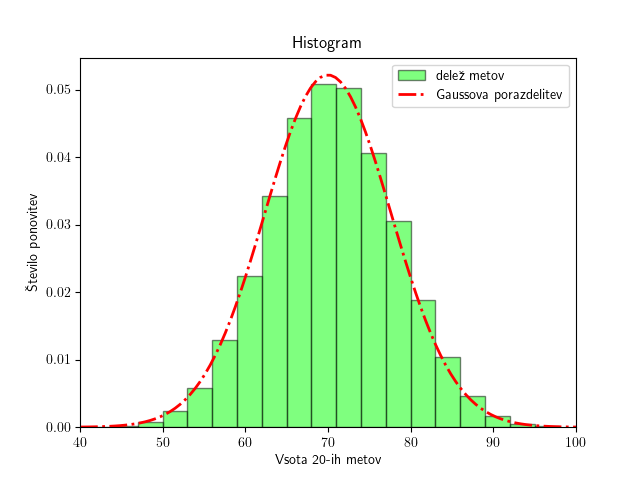
\includegraphics[width=10cm]{h.png}
    \caption{Porazdelitev vsote metov 20-ih kock}
    \label{histogram}
\end{figure}

\newpage
\section{$\bm{\mu}$ in $\bm{\sigma^2}$ pri poskusu}
Z $\mu$ pri Gaussovi označujemo povprečno vrednost. Z večanjem števila ponovitev se praviloma le-ta vedno bolj približuje pričakovani vrednosti. Pri vsoti 20-ih metov kocke bi pričakovali, da je ta vrednost ravno na sredini med maksimalno in minimalno vrednostjo, torej 70. V našem poskusu vrednost ne odstopa veliko od pričakovane, saj je le-ta 69.9909. Ko smo isti poskus ponovili z večjim številom ponovitev(500.000), se je vrednost še bolj približala pravi-69.994904. Ko smo poskus ponovili s samo 10.000 meritvami, pa je povprečje po pričakovanju bolj odstopalo od prave vrednosti, in sicer je bilo 70.0465.

S $\sigma^2$ pa označujemo standardni odklon. V interval $2\sigma$ pade približno 70 \% meritev. Z večanjem števila ponovitev se odklon praviloma manjša. V našem primeru ima $\sigma$ vrednost 7.64535. Ko smo poskus ponovili s 500.000 ponovitvami, se je le-ta po pričakovanjih zmanjšal na 7.63957.


\end{document}
